%\begin{tcolorbox}[
%    enhanced,
%    colback=ODD1!5,             % Fond léger
%    colframe=ODD1!80!black,     % Bordure
%    boxrule=0pt,                % Pas de contour épais
%    borderline west={3pt}{0pt}{ODD01}, % Bande colorée à gauche
%    left=5mm, right=5mm, top=2mm, bottom=2mm,
%    sharp corners
%]
%    \begin{minipage}{0.15\textwidth}
%        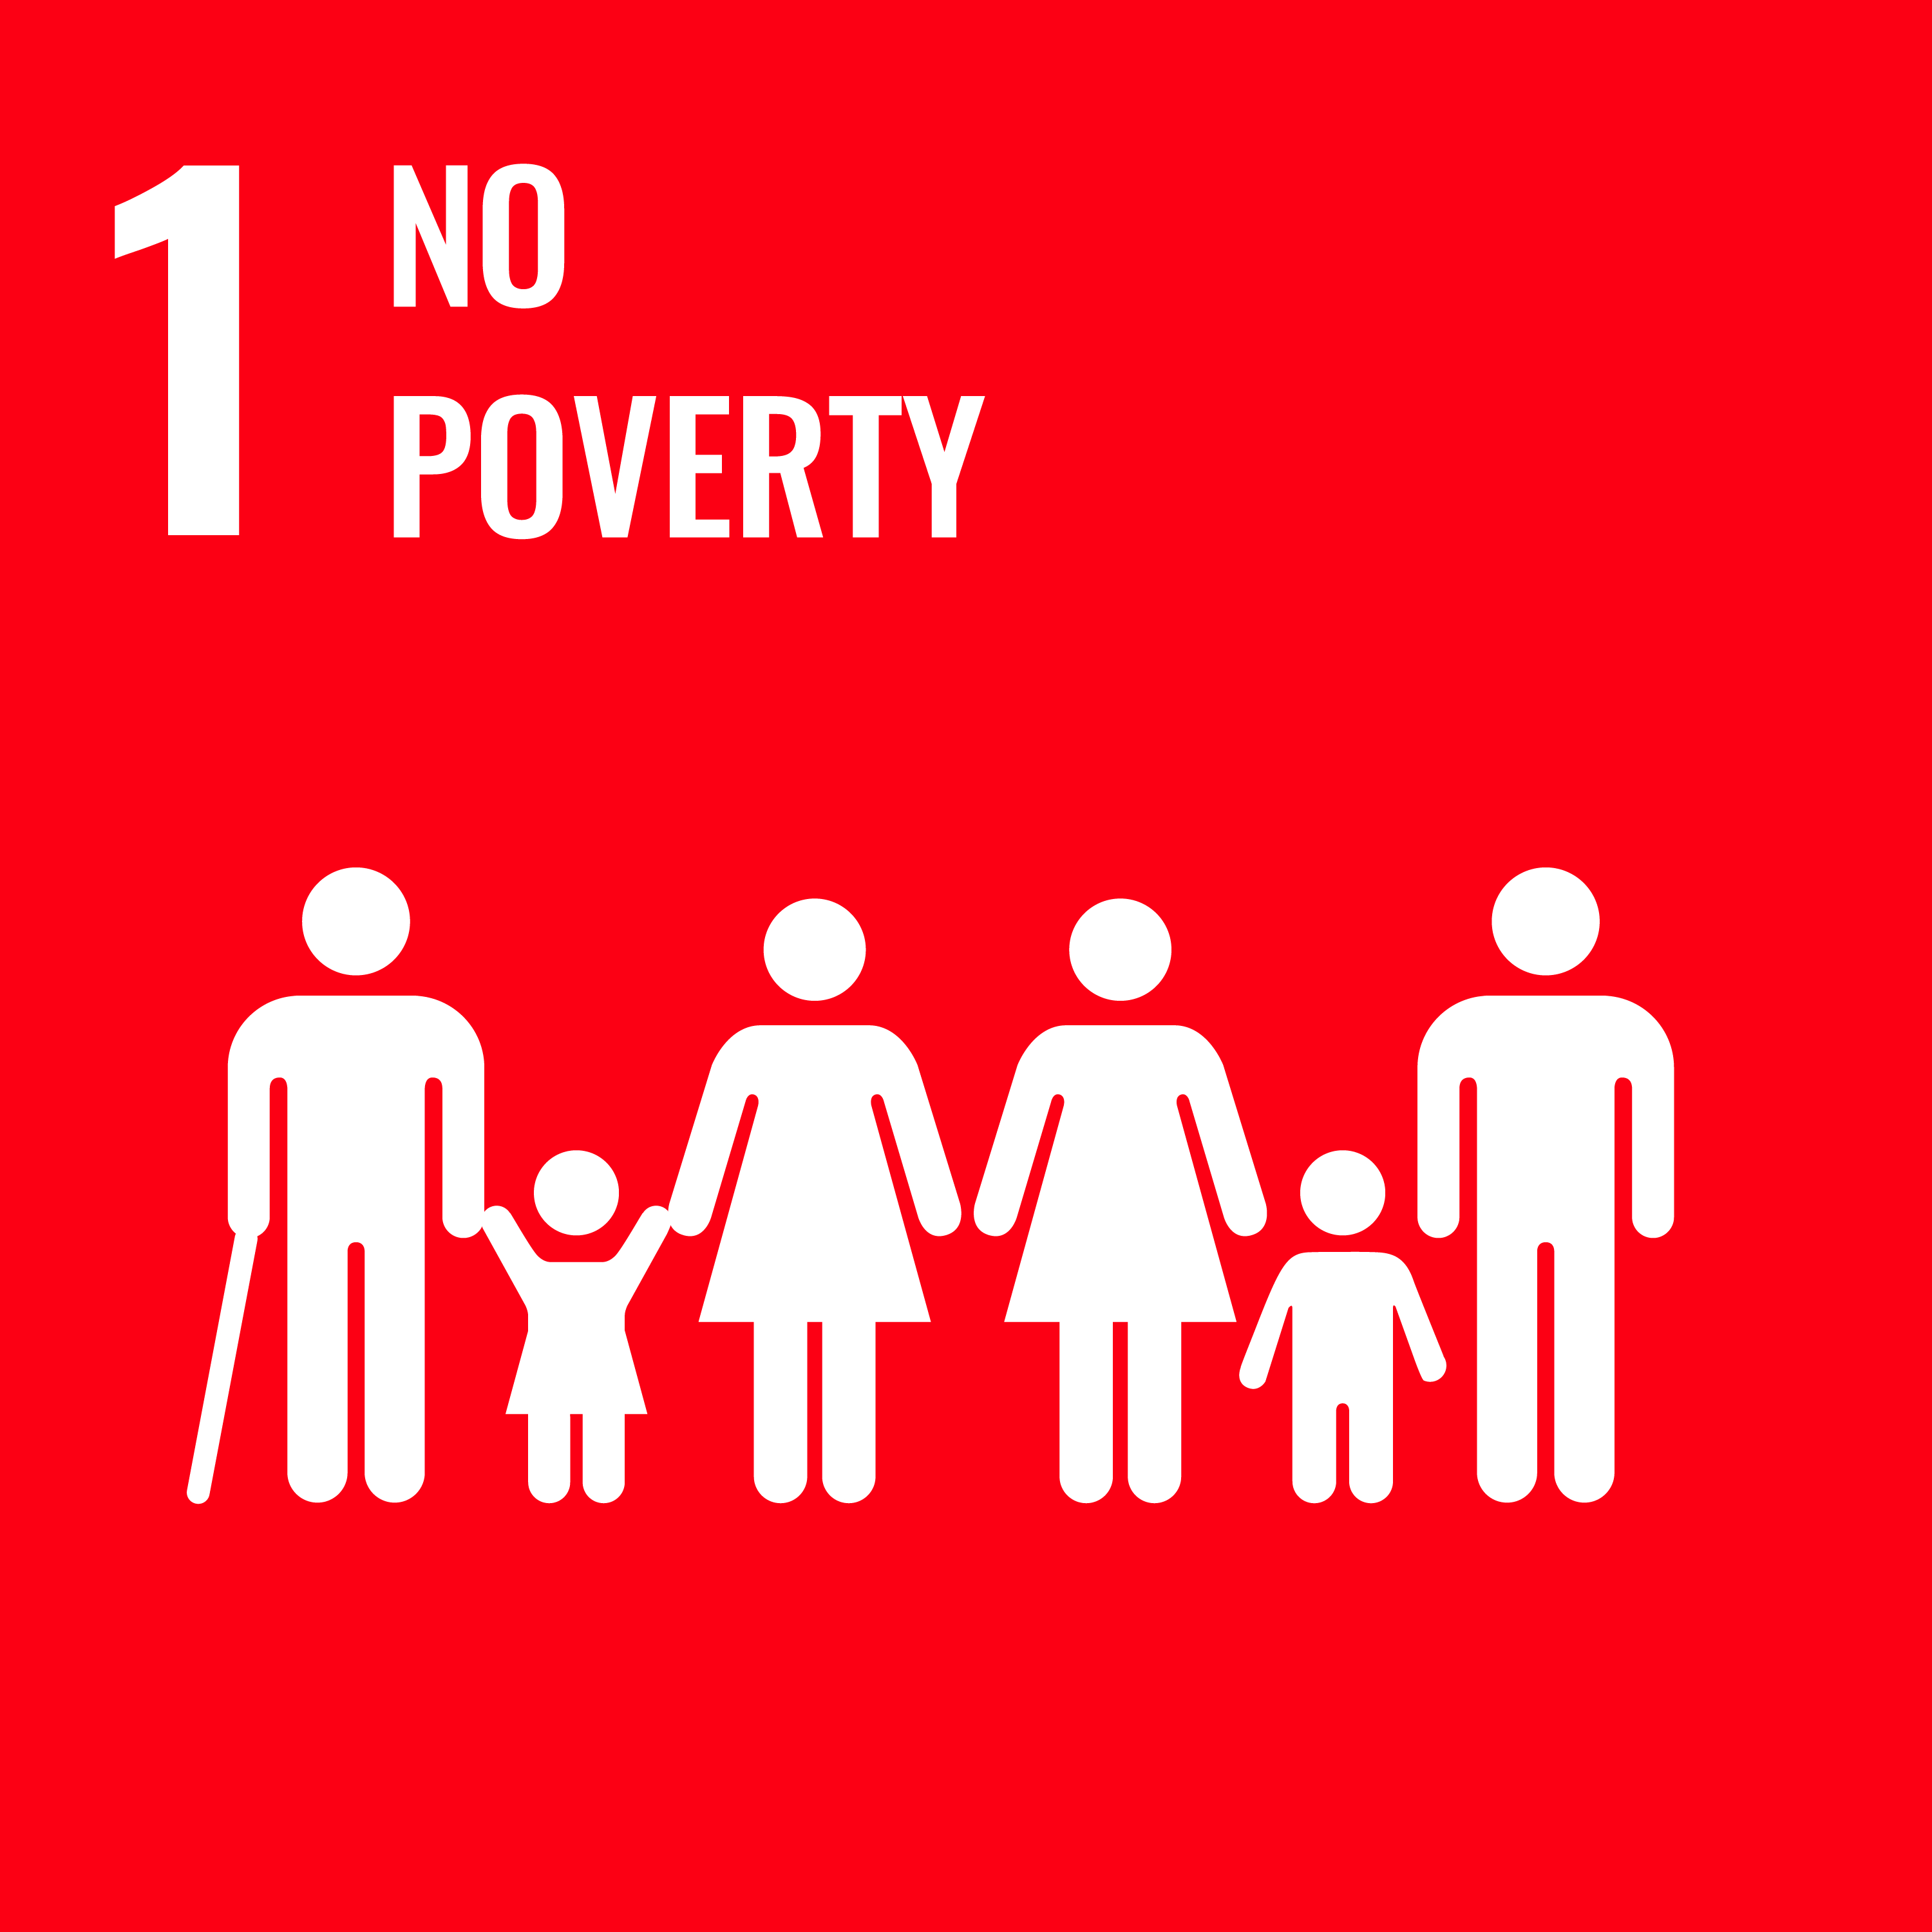
\includegraphics[width=\linewidth]{Pictures/ODD/ODD01.jpg}
%    \end{minipage}
%    \hfill
%    \begin{minipage}{0.8\textwidth}
%        {\bfseries\Large ODD 1 : Pas de pauvreté}\\[2pt]
%        \textit{Éliminer l’extrême pauvreté pour tous d’ici 2030}
%    \end{minipage}
%\end{tcolorbox}
%
%\vspace{0.4cm}
%
%% 👉 Exemple de contenu
%Dans ce cadre, nous analysons la situation du Sénégal par rapport aux cibles :
%\begin{itemize}
%    \item Réduire à 0\% la proportion de population vivant avec moins de 1,90 USD/jour.
%    \item Étendre les systèmes de protection sociale.
%    \item Garantir l’accès universel aux ressources économiques.
%\end{itemize}


\begin{simplebox2}
	
	\begin{minipage}{0.15\textwidth}
		        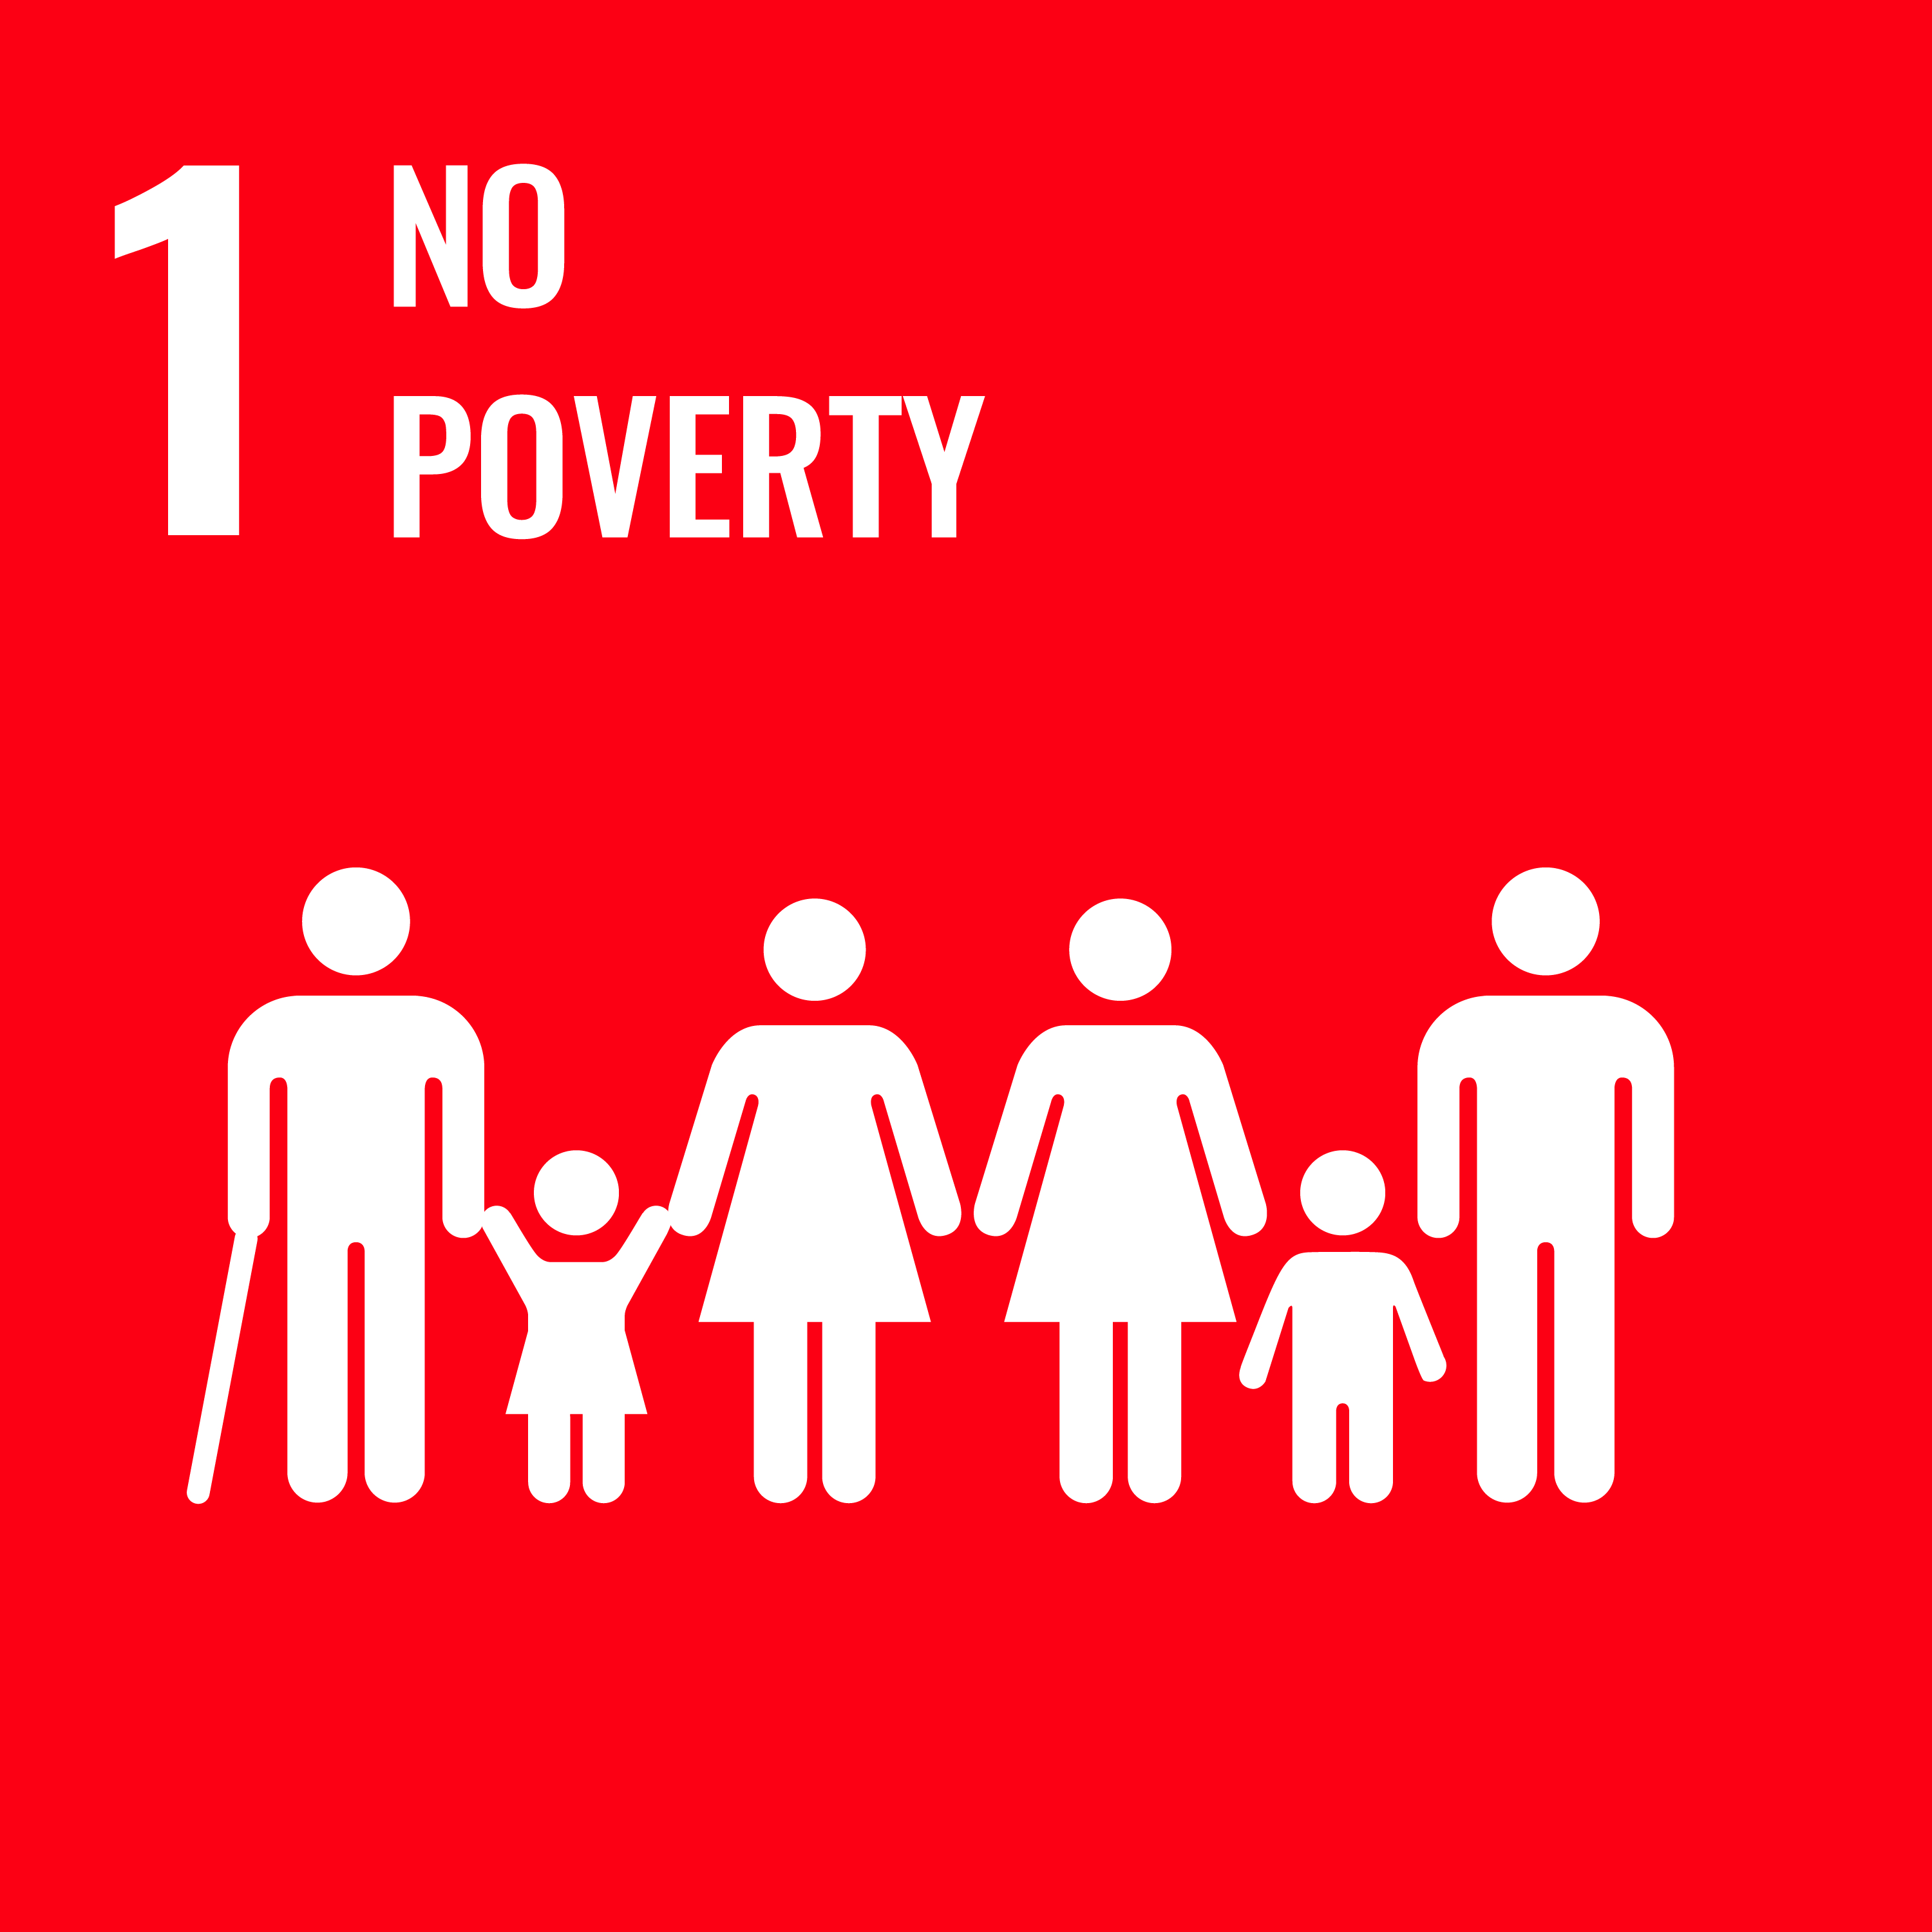
\includegraphics[width=\linewidth]{Pictures/ODD/ODD01.jpg}
		    \end{minipage}
		    \hfill
		    \begin{minipage}{0.8\textwidth}
		        {\bfseries\Large ODD 1 : Pas de pauvreté}\\[2pt]
		        \textit{Éliminer la pauvreté sous toutes ses formes et partout dans le monde}
		    \end{minipage}
\end{simplebox2}

\begin{simplebox}
	Réduire de moitié au moins la proportion d’hommes, de femmes et 
	d’enfants de tous âges souffrant d’une forme ou l’autre de pauvreté, 
	telle que définie par chaque pays.
\end{simplebox}

% ========================
% Section Pauvreté Sénégal
% ========================
\section*{Cible 1.2 : Réduction de la pauvreté}

L’éradication de la pauvreté sous toutes ses formes constitue un des défis majeurs des politiques nationales de développement : le \textbf{Plan Sénégal Émergent (PSE 2014-2018)}, le \textbf{PSE Phase II (2019-2023)} et le \textbf{Plan d’action pour la stabilisation et le développement (PA-SD 2023-2025)}.


Les différents référentiels nationaux ont permis de réduire progressivement la pauvreté. Selon les résultats de l’Enquête harmonisée sur les conditions de vie des ménages (EHCVM) :  

\begin{itemize}
	\item 2011 : incidence de la pauvreté à 46,7\%
	\item 2019 : incidence de la pauvreté à 37,4\%
	\item 2022 : incidence de la pauvreté à 37,5\%
\end{itemize}

L’EHCVM établit une base de référence cohérente pour la mesure et le suivi de la pauvreté. Sur cette base, la population pauvre représente environ 37,5\% de la population nationale, ce qui montre une progression mais indique que la pauvreté reste encore significative au Sénégal.

Le niveau de pauvreté demeure particulièrement marqué dans certaines régions et chez certains ménages. La pauvreté touche plus fortement les ménages ruraux et ceux dirigés par des hommes. L’incidence de la pauvreté monétaire pour les ménages dirigés par des hommes est généralement plus élevée que pour ceux dirigés par des femmes, et la pauvreté alimentaire suit la même tendance.

% ------------------------
% Insérer le graphique
% ------------------------
\begin{figure}[H]
	\centering
	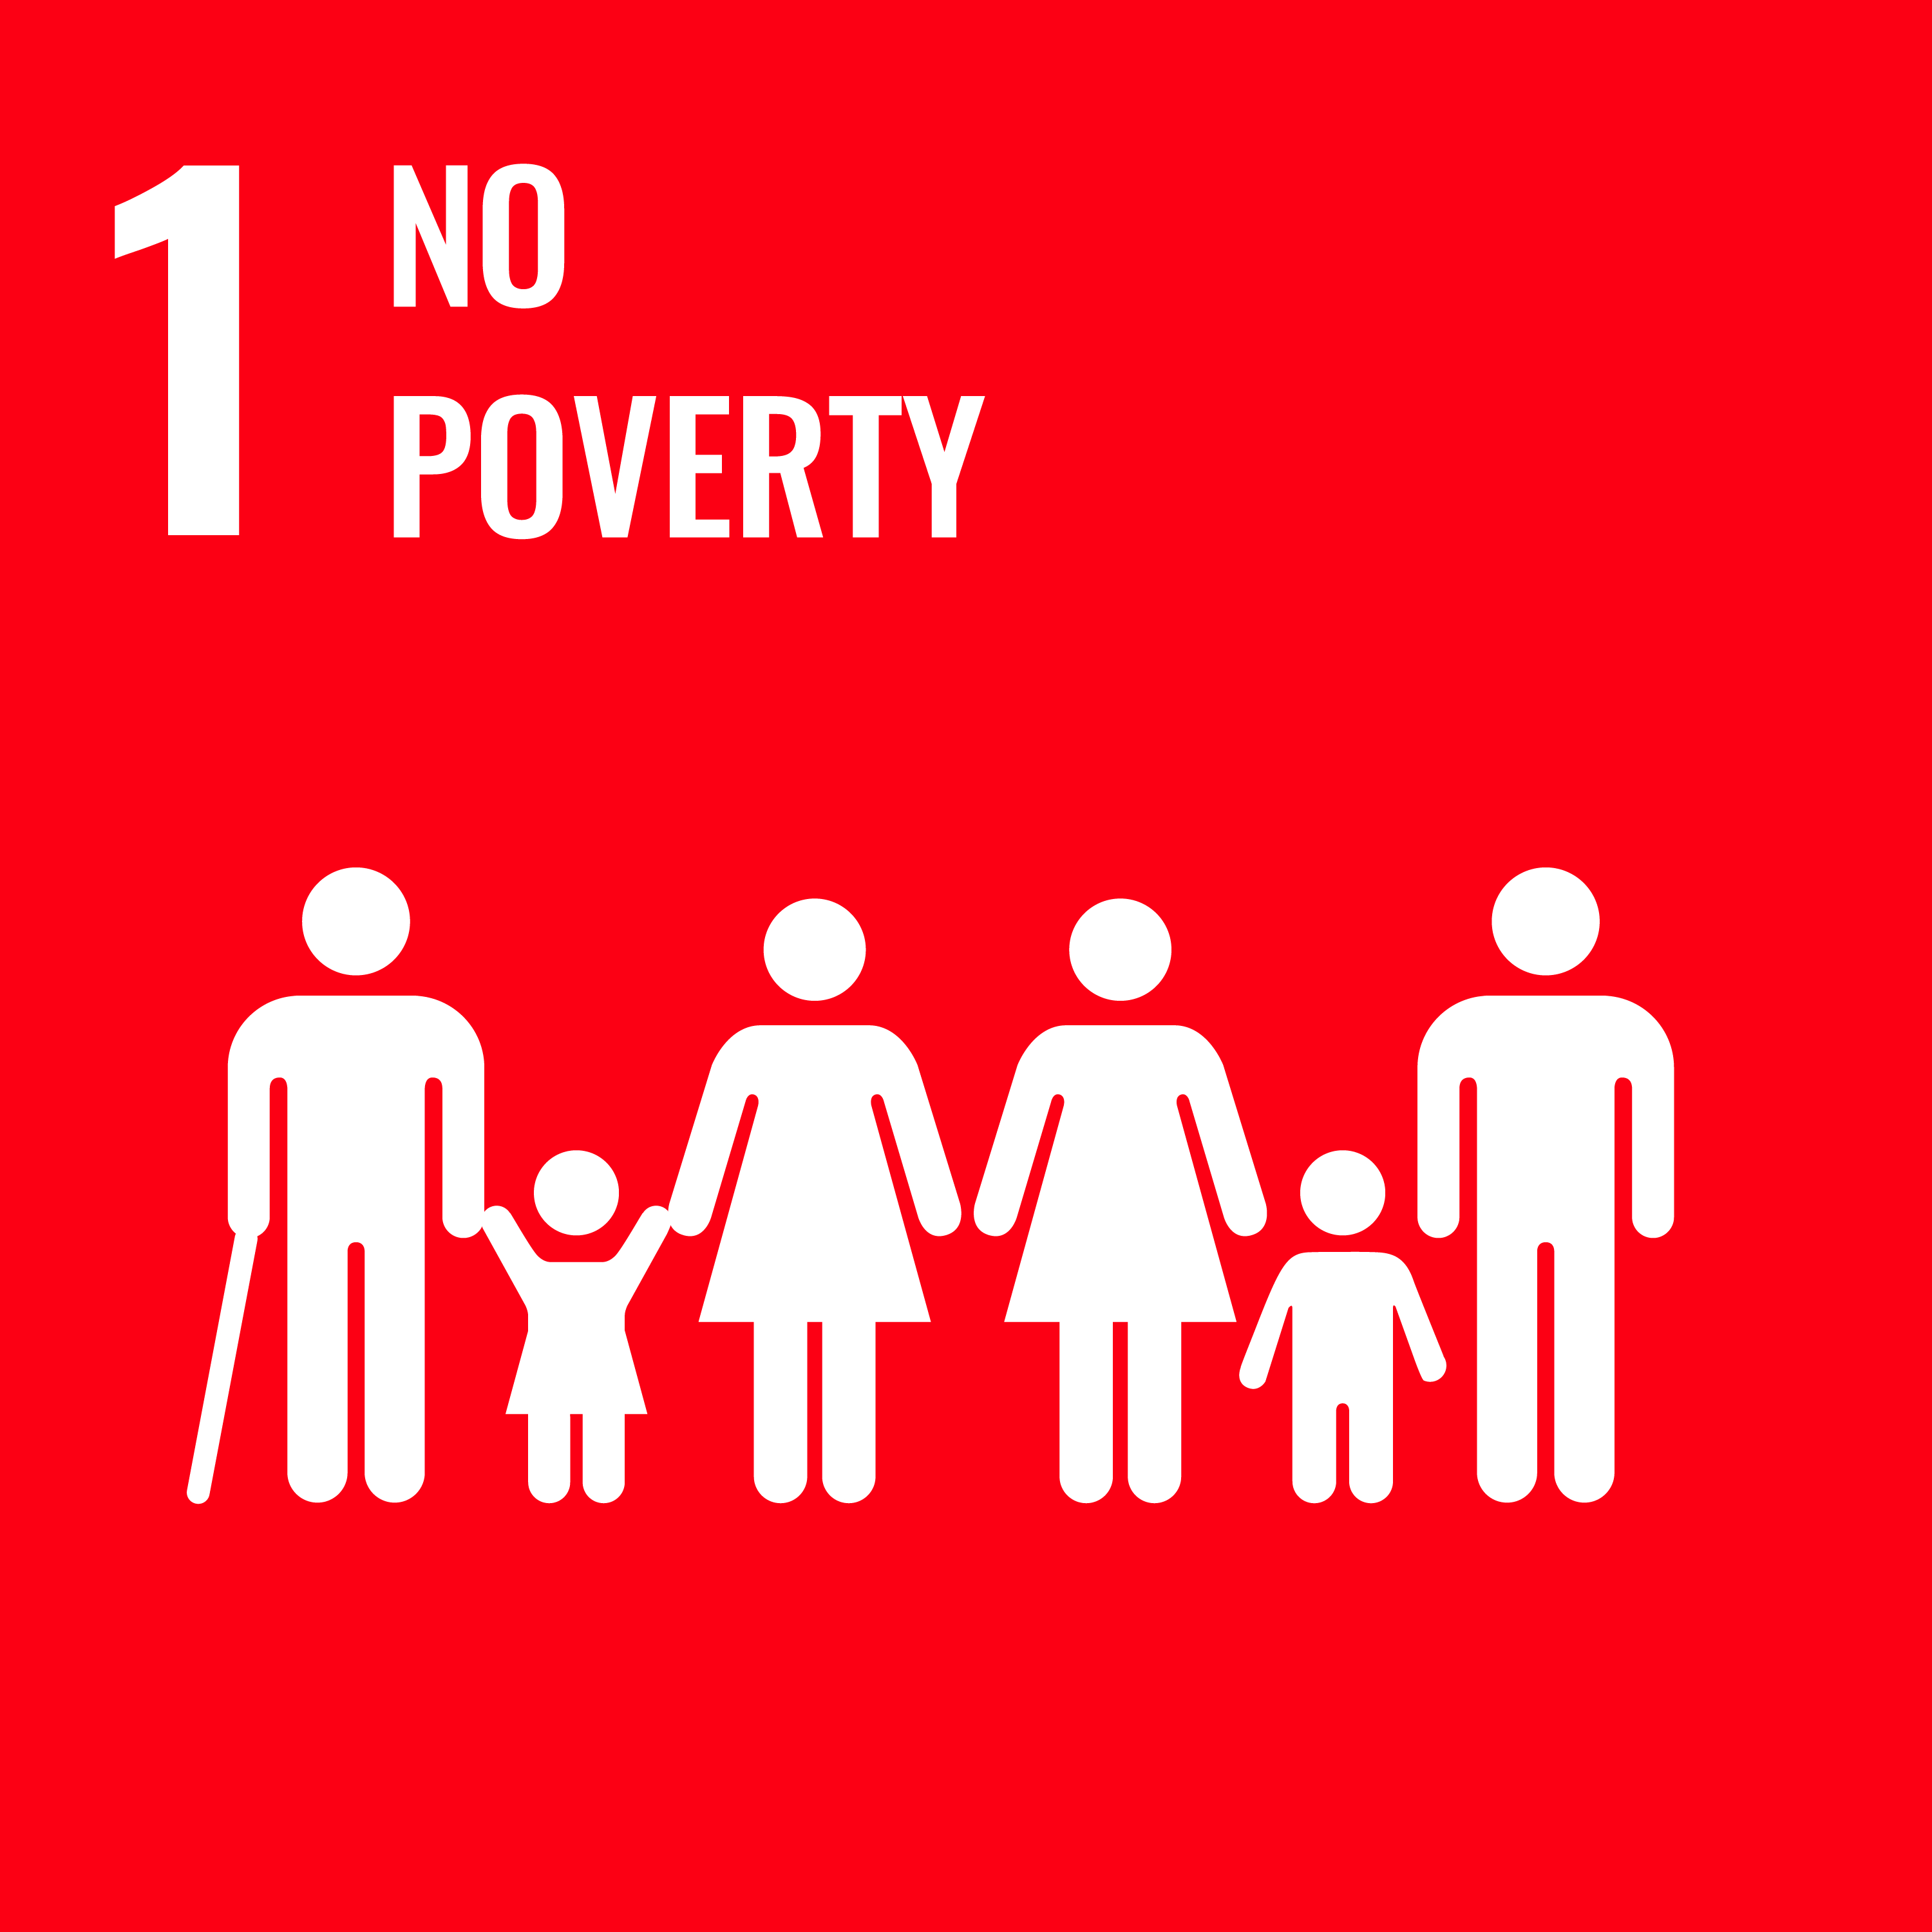
\includegraphics[width=0.7\textwidth]{Pictures/ODD/ODD01.jpg}
	%\caption{Évolution du taux de pauvreté au Sénégal (EHCVM 2011-2022)}
\end{figure}
